\subsection{Fundaments of the four color theorem}

The proof of the four color theorem follows the same structure as the five color theorem. We show that every planar graph contains a subgraph that allows us to reduce the coloring problem to a smaller graph. With \textit{smaller} we mean less vertices.

\begin{definition}
    The size $|G|$ of a graph is the number of vertices of $G$.
\end{definition}

\begin{definition}
    A graph $H$ is smaller than $G$ or $H < G$ if $|H| < |G|$.
\end{definition}

This notion of a \textit{subgraph} of a graph requires some extra attention, since we will need a stronger notion of being a subgraph called \textit{containment}. See Figure \ref{fig:containtut}. The graphs $\confg$ contained in others that we use for reducibility purposes, are called \emph{configurations}.

\begin{figure}[!ht]
    \centering
    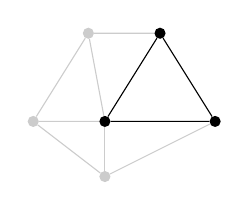
\begin{tikzpicture}[scale=0.7]
        \node[circle, fill, scale=0.015cm] (l1) at (-1, 0) { };
        \node[circle, fill, scale=0.015cm] (l2) at (1, 0) { };
        \node[circle, fill, scale=0.015cm] (l3) at (0, 1.6) {};

        \node[circle, fill, scale=0.015cm, opacity=0.2] (e1) at (-1.3, 1.6) { };
        \node[circle, fill, scale=0.015cm, opacity=0.2] (e2) at (-2.3, 0) { };
        \node[circle, fill, scale=0.015cm, opacity=0.2] (e3) at (-1, -1) { };

        \draw (l1) -- (l2) -- (l3) -- (l1);
        \draw[opacity=0.2] (e1) -- (l1) -- (e2);
        \draw[opacity=0.2] (e3) -- (l1);
        \draw[opacity=0.2] (l3) -- (e1) -- (e2) -- (e3) -- (l2);
    \end{tikzpicture}
    \hspace{1cm}
    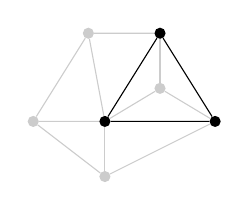
\begin{tikzpicture}[scale=0.7]
        \node[circle, fill, scale=0.015cm] (l1) at (-1, 0) { };
        \node[circle, fill, scale=0.015cm] (l2) at (1, 0) { };
        \node[circle, fill, scale=0.015cm] (l3) at (0, 1.6) {};

        \node[circle, fill, scale=0.015cm, opacity=0.2] (e1) at (-1.3, 1.6) { };
        \node[circle, fill, scale=0.015cm, opacity=0.2] (e2) at (-2.3, 0) { };
        \node[circle, fill, scale=0.015cm, opacity=0.2] (e3) at (-1, -1) { };

        \node[circle, fill, scale=0.015cm, opacity=0.2] (w1) at (0, 0.6) { };

        \draw (l1) -- (l2) -- (l3) -- (l1);
        \draw[opacity=0.2] (w1) -- (l1);
        \draw[opacity=0.2] (w1) -- (l2);
        \draw[opacity=0.2] (w1) -- (l3);
        \draw[opacity=0.2] (e1) -- (l1) -- (e2);
        \draw[opacity=0.2] (e3) -- (l1);
        \draw[opacity=0.2] (l3) -- (e1) -- (e2) -- (e3) -- (l2);
    \end{tikzpicture}
    \caption{A configuration contained in a graph (left). No containment (right).}
    \label{fig:containtut}
\end{figure}

\begin{definition}
    A planar graph $\confg$ is \emph{contained} in a graph $G$, if $G\setminus \confg$ (removed $\confg$) is connected.
\end{definition}

\begin{definition}
    A planar graph $\confg$ is \emph{reducible} in a graph $G$, if $\confg$ being contained in $G$ implies that there exists graphs $H < G$ called \emph{reductions} whose 4-colorings can be used to 4-color $G$.
\end{definition}

Therefore, in a reducibility proof, we may assume that any graph $H$ smaller than $G$ is 4-colorable. Then, we show that a 4-coloring of $H$ can be extended to a 4-coloring of $G$.
Using these two definitions we can formulate the key theorem of the four color theorem. We proved the same result for the five color theorem.

\begin{theorem}
    \label{funda1}
    Every planar graph $G$ contains a configuration $\confg$ that is either $k$-reducible, D-reducible or C-reducible in $G$.
\end{theorem}

From this theorem, a 4-coloring of a planar graph $G_0$ can be found as follows. This is the same procedure that we used for the vertex of $\deg(v)\leq 5$ in the five color theorem.

\begin{enumerate}
    \item Find a reducible configuration $C_n$ in $G_n$.
    \item Reduce the graph $G_n$ to the smaller graph $G_{n+1}$.
    \item If $G_{n+1}$ is the empty graph, color all the intermediate graphs starting from $G_n$ all the way until $G_0$. Else, repeat Step 1 on $G_{n+1}$.
\end{enumerate}

There are many ways to prove that a configuration is reducible. We will be treating the three central forms of reducibility that are used in the four color theorem. Each of them allows us to test the reducibility of certain configurations. These forms of reducibility are by no means perfect, each has its flaws and uses. A single, most general definition of reducibility is still not found. If such a single form would exist, then it would capture the heart of the four color problem.